%%%%%%%%%%%%%%%%%%%%%%%%%%%%%%%%%%%%%
%%%%%%%%%% Plantilla del Team para el proyecto final 
%%%%%%%%%%%%%%%%%%%%%%%%%%%%%%%%%%%%%
%%%%%%%%%% Nueva clase personalizada
\documentclass{staprojteamusb}
%%%%%%%%%% Nuevo estilo personalizado
\usepackage{staprojteamusbsty}

\addbibresource{referencias.bib}
%%%%%%%%%%%%%%%%%%%%%%%%%%%%%%%%%%%
%%%%%%%%%% Variables de Markdown
%%%%%%%%%%%%%%%%%%%%%%%%%%%%%%%%%%%
%%%%%%%%%% Encabezado 
\titulo{Análisis estadístico sobre una base de datos de beísbol.}

\autor{
		Eduardo Gavazut\\
	Universidad Simón Bolívar \\
	Caracas, Venezuela \\
	\texttt{\href{mailto:13-10524@usb.ve}{\nolinkurl{13-10524@usb.ve}}} \\
	 \And
		Luis Riera\\
	Universidad Simón Bolívar \\
	Caracas, Venezuela \\
	\texttt{\href{mailto:16-10976@usb.ve}{\nolinkurl{16-10976@usb.ve}}} \\
	 \And
		Miguel Cordero\\
	Universidad Simón Bolívar \\
	Caracas, Venezuela \\
	\texttt{\href{mailto:15-10326@usb.ve}{\nolinkurl{15-10326@usb.ve}}} \\
	}
\fecha{8 de abril de 2022}
\resumen{En este documento se trata la descripción de los datos, la
clase de la base de datos y los estadísticos para las variables}

\palabrasc{}
%%%%%%%%%%%% Resto de las variables propias de R eso viene por defecto de R


%%%%%%%%% Estilo de las listas sin salto de linea
\providecommand{\tightlist}{%
	\setlength{\itemsep}{0pt}\setlength{\parskip}{0pt}}


%%%%%%%%%%%% Si hay paquetes por incluir en header-include
%%%%%%%%%%%%%%%%%%%%%%%%%%%%%%%%%%%%%%%%%%%%%%%%%%%%%%%%%
\begin{document}
	
	
	\maketitle
	
	%%%%%%%%%%%% Si hay cosas que incluir en include-before
		%%%%%%%%%%%%%%%%%%%%%%%%%%%%%%%%%%%%%%%%%%%%%%%%%%%%%%%%%
	
	%%%%%%%%%%%%% Inicio del documento
	
	\hypertarget{planteamiento-del-problema}{%
 \section{Planteamiento del problema}\label{planteamiento-del-problema}}

 Se desea realizar un análisis estadístico completo sobre una base de
 datos con información sobre el rendimiento de algunos jugadores de
 beisbol y en particular estudiar la relación (si la hay) de los hits al
 bate respecto a las carreras, dobles, triples, jonrones y ponches de
 los jugadores.

 \hypertarget{metododologuxeda}{%
 \subsection{Metododología}\label{metododologuxeda}}

 Para la realización de esta investigación se hará uso del sofware
 estadístico \texttt{R} en el entorno de desarrollo intergrado (IDE)
 \texttt{RStudio}. En este se iniciará por una descripción de los datos
 y variables almacenadas en el archivo fuente \emph{Baseball.xlsx},
 tales como: mínimo, media, cuantiles y desviación estándar. Para la
 media de las variables se obtendrá un intervalo de confianza del
 \(95\%\). Como se desea estudiar la relación de la tasa de bateo
 respecto al resto de las variables, se buscará determinar la mejor
 distribución de probabilidad que se ajuste a esta variable. Finalmente,
 se estudiará la eficiencia del mejor modelo lineal de predicción que se
 ajuste a los datos y permita establecer si en efecto existe tal
 relación entre las variables y las implicaciones que tendría en las
 estrategias para futuros juegos de beisbol.

 \hypertarget{descripciuxf3n-de-los-datos}{%
 \section{Descripción de los datos}\label{descripciuxf3n-de-los-datos}}

 Para la realización de este proyecto se contó con una archivo de excel
 con la información de algunos jugadores de la Major League Beisbol o
 MLB, el cual se almacenó en una variable llamada \texttt{Baseball}:

 \hypertarget{realizar-un-anuxe1lisis-descriptivo-de-los-datos}{%
 \subsection{Realizar un análisis descriptivo de los
 datos}\label{realizar-un-anuxe1lisis-descriptivo-de-los-datos}}

 \hypertarget{quuxe9-clase-es-la-base-de-datos}{%
 \subsubsection{¿Qué clase es la base de
 datos?}\label{quuxe9-clase-es-la-base-de-datos}}

 Con el comando \texttt{class}, se pudo determinar el tipo de base de
 datos utilizada o lo que es equivalente, la clase de la variable
 \texttt{Baseball}.

 El resultado que se obtuvo indica que es del tipo \texttt{tbl\_df}, que
 es una subclase de la clase \texttt{data.frame}. \texttt{tbl\_df}
 cumple con tener propiedades diferentes por defecto y se suele referir
 a ellas como \texttt{tibble}. Es una clase eficiente para trabajar con
 bases de datos grandes y su visualización.

 \hypertarget{variables-en-la-base-de-datos}{%
 \subsubsection{Variables en la base de
 datos}\label{variables-en-la-base-de-datos}}

 Si se desea saber que tipo de variables están almacenadas en la base de
 datos, se puede utilizar el comando \texttt{str}. Esta función nos
 indica que se cuentan con \(6\) variables denominadas
 \texttt{X1,X2,X3,X4,X5,X6}, y distribuidas de tal manera que
 representan la columnas de la base de datos. Cada una de estas
 variables tienen \(45\) valores de tipo \texttt{double} o número
 decimal, que representan las \(45\) observaciones aleatorias (una por
 fila) realizadas a jugadores de la (MLB) .

 Cada variable representa la siguiente información:

 \begin{itemize}
 \tightlist
 \item
   \texttt{X1}: tasa de bateo, (hit/veces al bate).
 \item
   \texttt{X2}: tasa de carreras anotadas, (carreras anotadas/veces al
   bate).
 \item
   \texttt{X3}: tasa de dobles, (dobles/ veces al bate).
 \item
   \texttt{X4}: tasa de triples, (tripes/ veces al bate).
 \item
   \texttt{X5}: tasa de jonrones, (jonrones/ veces al bate).
 \item
   \texttt{X6}: tasa de ponches, (ponches/ veces al bate).
 \end{itemize}

 \hypertarget{estaduxedsticos}{%
 \subsubsection{Estadísticos}\label{estaduxedsticos}}

 Para obtener los estadísticos de las seis (6) variables de esta base de
 datos, se inicia por guardar las \(45\) observaciones en un vector que
 represente a cada variable.

 Con los datos vectorizados se pueden aplicar las siguientes funciones:
 \texttt{mean} que permite obtener la media de los datos,
 \texttt{median} para obtener la mediana, \texttt{quantile} retornar los
 cuantiles al \(0.25\%, 0.50\%\) y \(0.75\%\) de cada variable,
 \texttt{min} para el valor mínimo, \texttt{max} para el valor máximo,
 \texttt{var} para la varianza, \texttt{sd} desviación estándar,
 \texttt{IQR} es para el rango intercuartil y finalmente, el coeficiente
 de variación obtenido como \texttt{stad/media}.

 Podemos ver la información por cada variable en las siguientes tablas:

\begin{verbatim}
##    Minimo   25%  Media Mediana / 50  75% Máximo   RIC Varianza Desv. Estándar
## X1  0.188 0.248 0.2805         0.29 0.06  0.308 0.367   0.0019          0.044
## X2  0.064 0.119 0.1509         0.15 0.07  0.189 0.259   0.0018          0.042
##    Coef. Variación
## X1          0.1569
## X2          0.2784
\end{verbatim}

 De estos resultados hay varios puntos que podemos detacar. La varianza
 de los datos es muy baja indicativo que entre los datos no hay valores
 atípicos; la media y la mediana son casi idénticos, de hecho en la tasa
 de carreras anotadas se puede decir que coinciden, esto indica que hay
 cierta simetría en los datos recolectados; sin embargo, la diferencia
 entre el máximo y el mínimo para la tasa de bateo es casi el doble en
 comparación con la tasa de carreras anotadas.

 \hypertarget{diagramas-e-histograma-de-los-datos-por-cada-variable}{%
 \subsubsection{Diagramas e histograma de los datos por cada
 variable}\label{diagramas-e-histograma-de-los-datos-por-cada-variable}}

 \begin{figure}
 \centering
 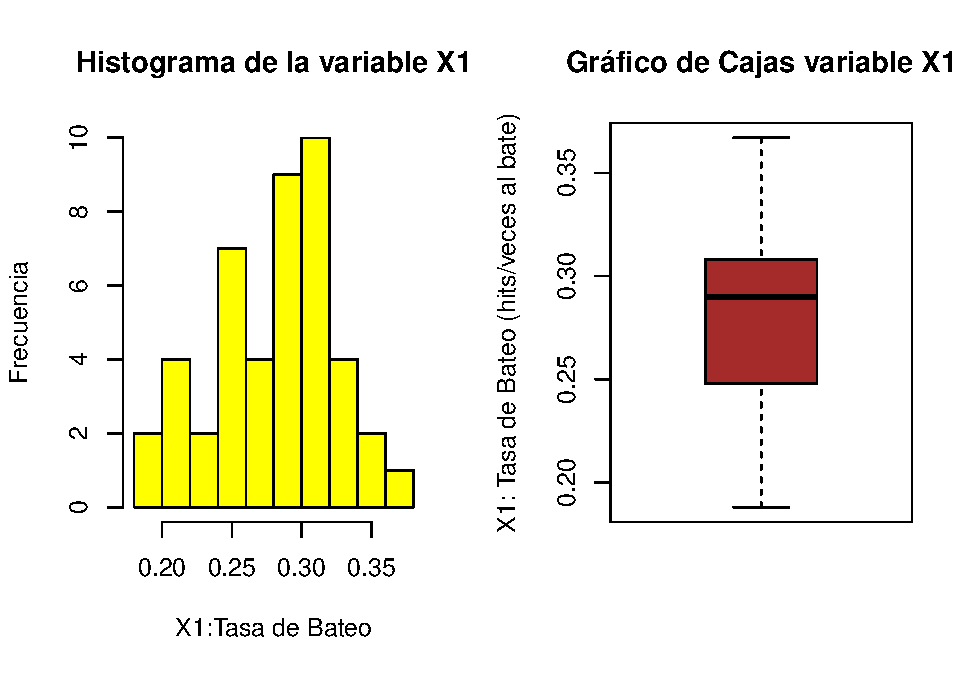
\includegraphics{Descripcion-Datos_files/figure-latex/unnamed-chunk-7-1.pdf}
 \caption{Histograma y gráfico de cajas para las variables X1}
 \end{figure}

 De la gráfica para la variable X1 podemos ver como los valores máximos
 de los datos se obtienen luego de la media, pero el mayor volumen de
 ellos se encuentra antes como bien se observa en el diagrama de caja
 que permite confirmar la ausencia de datos atípicos.

 \begin{figure}
 \centering
 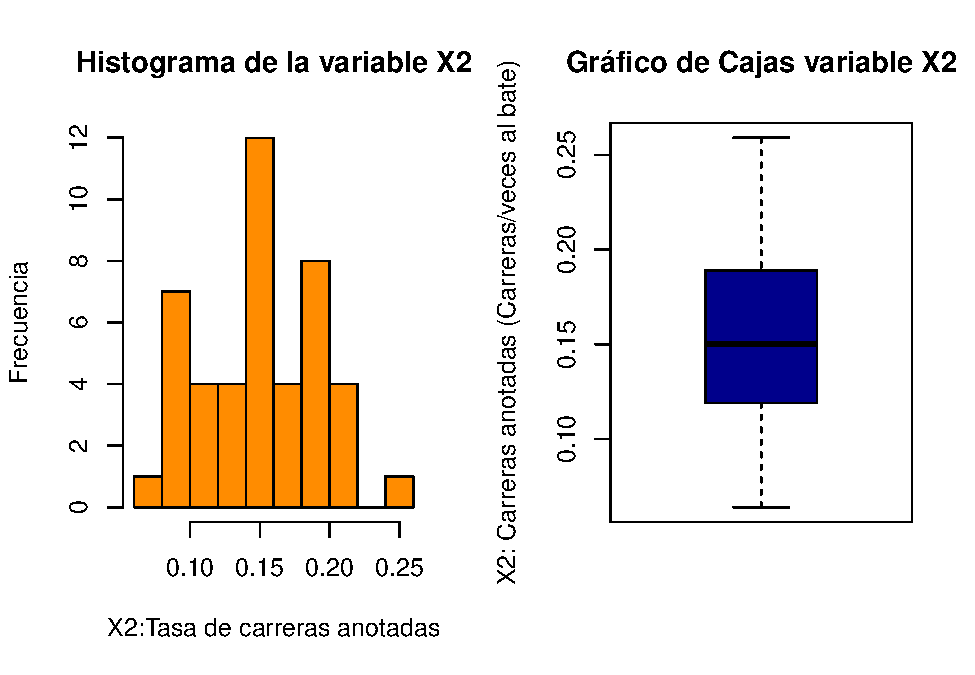
\includegraphics{Descripcion-Datos_files/figure-latex/unnamed-chunk-8-1.pdf}
 \caption{Histograma y gráfico de cajas para las variables X2}
 \end{figure}

 De la gráfica para la variable X2 podemos ver la simetría que se
 infería de la tabla anterior, con respecto al valor \(0.15\) que
 coincide a su vez con la media de los datos. El diagrama de caja
 permite confirmar la ausencia de los valores atípicos.
	
	%%%%%%%%%%%%% Fin del documento
	
	%%%%%%%%%%%% Inicio de la bibliografia
	
	\printbibliography
	
	
	%%%%%%%%%%%%% Fin de la bibliografia
	
	%%%%%%%%%%%%%%%%% Si hay cosas que incluir en include-after
		%%%%%%%%%%%%%%%%%%%%%%%%%%%%%%%%%%%%%%%%%%%%%%%%%%%%%%%%%%%%
	
\end{document}
